%\documentclass{article}
\documentclass[border=5pt]{standalone}
\usepackage{tikz}
\usetikzlibrary{decorations.markings,decorations.pathreplacing,calc}

\tikzset{help lines/.style={very thin,color=gray!50}} % modify the help lines style
\tikzset{->-/.style={decoration={
  markings,
  mark=at position .5 with {\arrow{>}}},postaction={decorate}}}
  
\begin{document}

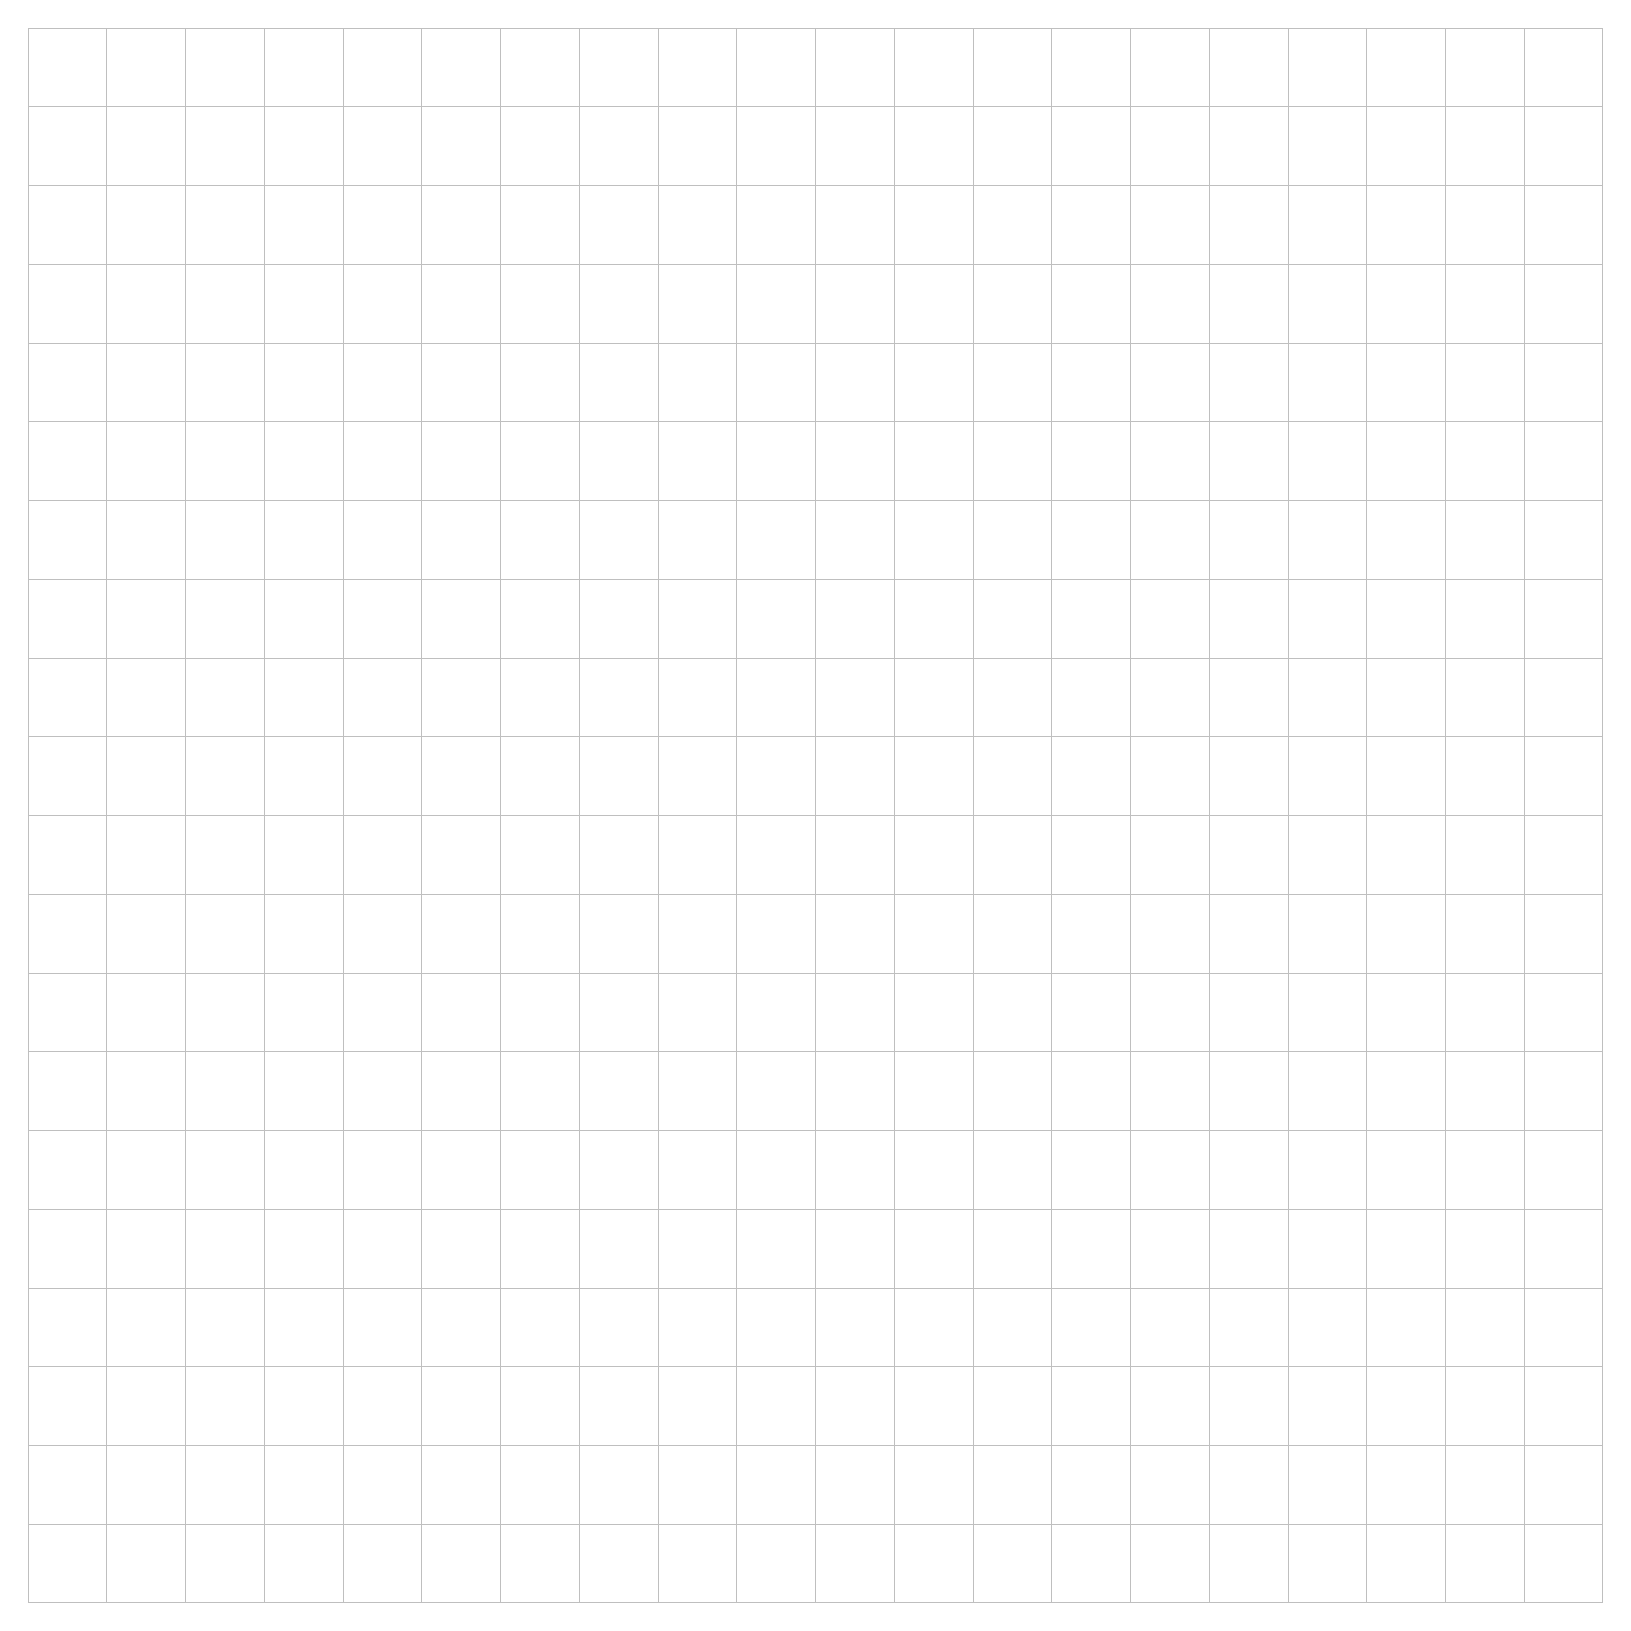
\begin{tikzpicture}[scale=1]
	\draw[help lines] (-10,-10) grid (10,10); %grid
	
\end{tikzpicture}
\end{document}